\section{Centroid Redundant Symbols}
\label{sec:sac}

Assume that we partition the grid in $n \times n$ areas, with $n$ an odd number.
Figure~\ref{fig-grid} shows an example, with a few $3 \times 3$ areas shown with thick lines.
The node at the middle of a given area is called the centroid of that area.
Consider a node $P$ in a given area with the centroid $C_1$.
Consider further a source node $S$.
If a first optimal move from $S$ towards $P$ coincides with a first optimal
move from $S$ towards $C_1$, then we can add a redundant $\gamma$ symbol
in the cell of the first-matrix move correspondig to row $S$ and column $P$.

Assume that, in our ordering of the columns of the first-move matrix,
nodes $P,R,Q$ came in this order.
As Figure~\ref{fig-row-1}, a standard CPD would not allow to compress together
the three consecutive symbols corresponding to row $S$ and columns $P,R,Q$.
On the other hand, Figure~\ref{fig-row-2} shows that we can add the $\gamma$ symbol
in all these three cells.
The reason is the following: a first move from $S$ towards $P$ coincides with a first move from $S$ towards $C_1$;
a first move from $S$ towards $R$ coincides with a first move from $S$ towards $C_3$;
and a first move from $S$ towards $Q$ coincides with a first move from $S$ towards $C_2$.
Now we can better compress the corresponding sequence.

Centroid redundant moves should be used with a lower priority than default moves.
I.e., it could happen that in two consecutive cells of a given matrix row,
we have both a default move symbol and a $\gamma$ symbol.
Then we should encode the default-move symbol.
The reason is that using $\gamma$ symbols may require two binary searches.
Indeed, consider a source $S$, a target $T$, and the centroid of the target, $C$.
If we encoded the move towards $T$ as $\gamma$,
then the first binary search
will discover that the $\gamma$ symbol is encoded; then we search again
for the move to the centroid $C$, which is also an optimal move towards $T$.

\begin{figure}[tb]
	\centering
	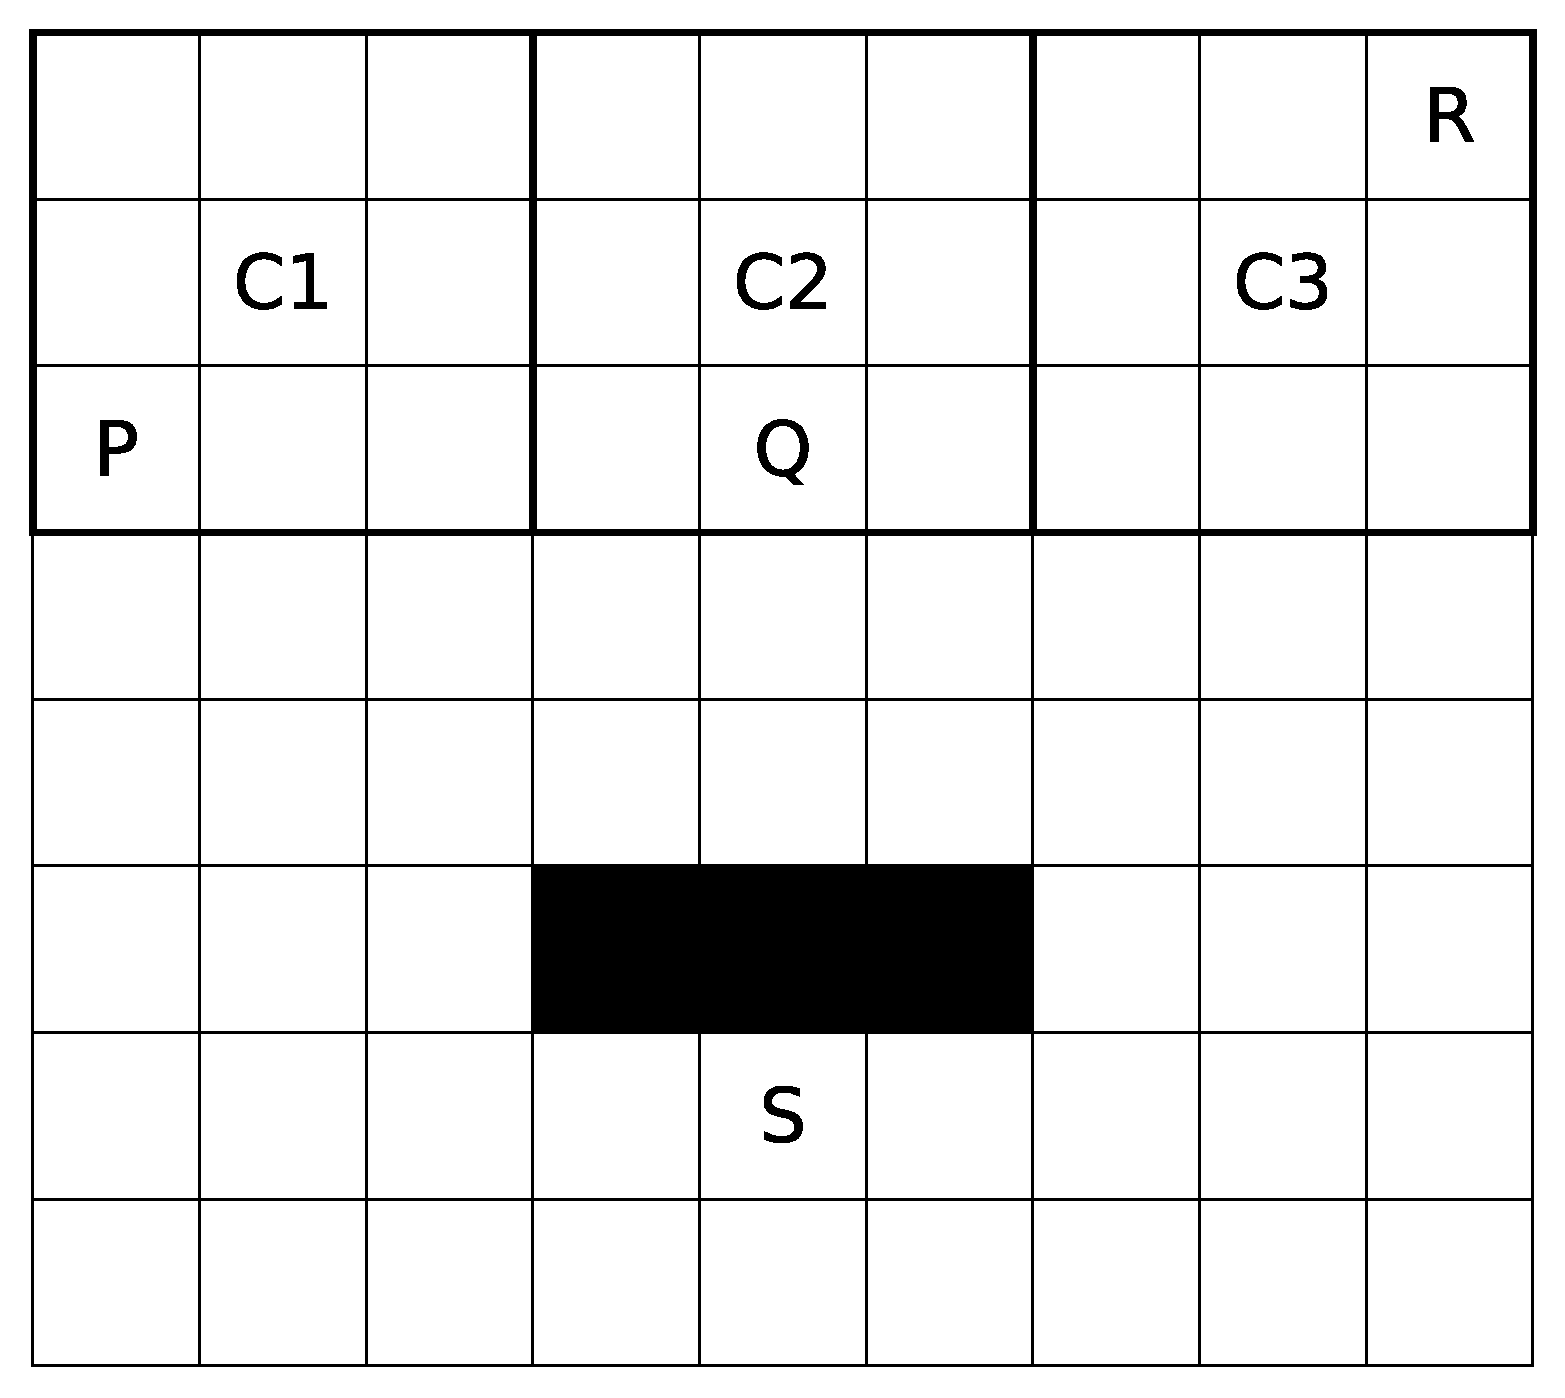
\includegraphics[width=.5\columnwidth]{gridmap.pdf}
	\caption{A toy gridmap used as an example.}
	\label{fig-grid}
\end{figure}


\begin{figure}[tb]
	\centering
	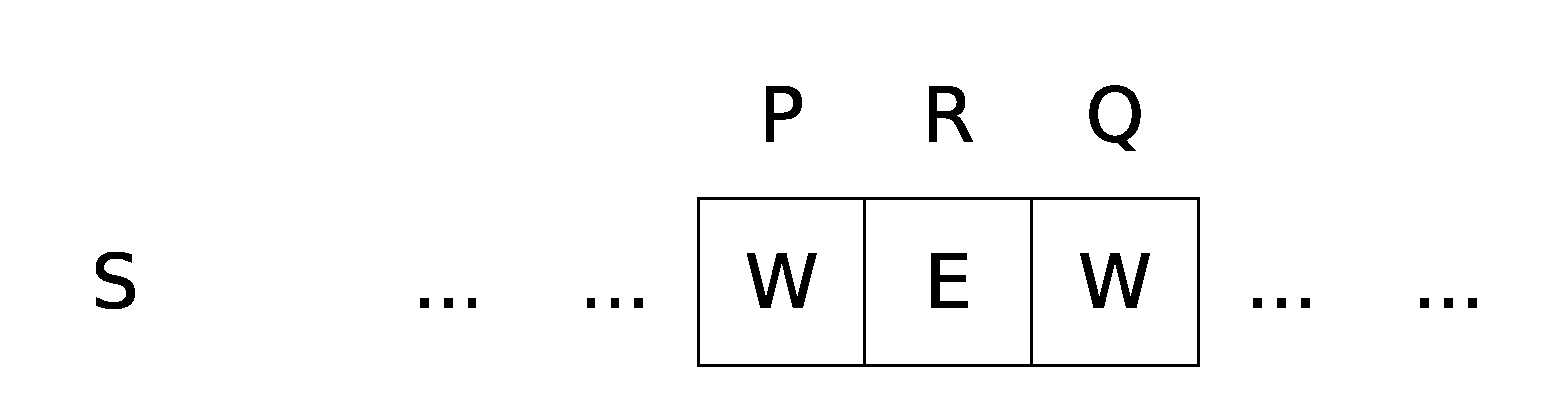
\includegraphics[width=.5\columnwidth]{rows.pdf}
	\caption{A few cells in the row of $S$ in a standard CPD (before compression).}
	\label{fig-row-1}
\end{figure}


\begin{figure}[tb]
	\centering
	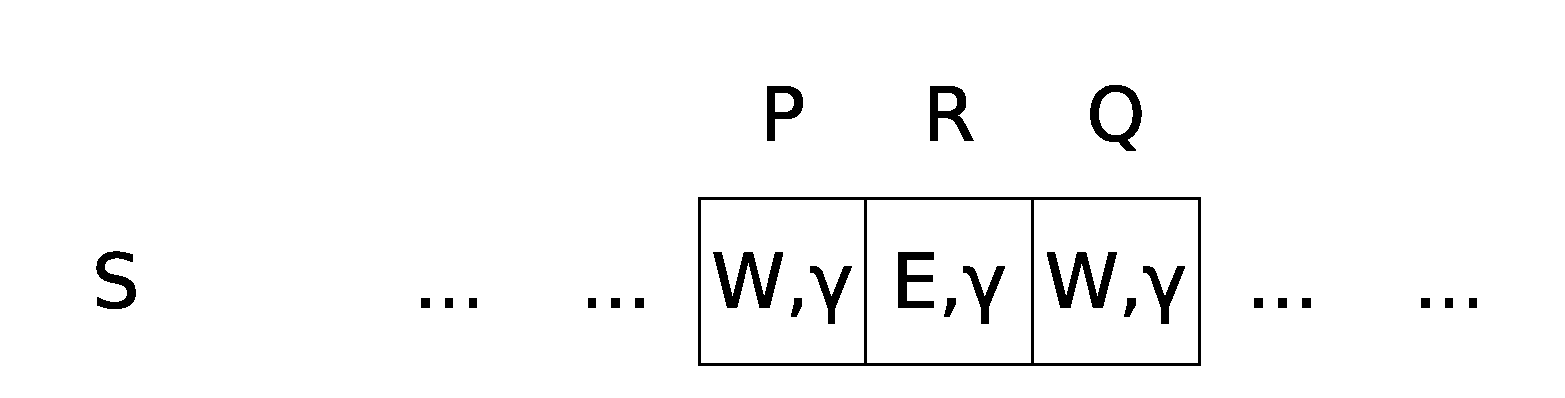
\includegraphics[width=.5\columnwidth]{rows2.pdf}
	\caption{A few cells in the row of $S$ in a CPD with $\gamma$ redundant symbols (before compression).}
	\label{fig-row-2}
\end{figure}


